\chapter{Formal Analysis using Alloy}
\label{chap:Formal-Analysis-using-Alloy}

\par
This chapter presents the formal modeling and verification of the \textit{Best Bike Paths} (BBP) system using the Alloy specification language and the Alloy Analyzer. The purpose of this analysis is to complement the natural language requirements and semi-formal UML diagrams with a precise, analyzable model.

\par
Alloy is employed here as a lightweight formal method to reason about the system's structure and critical behaviors. Specifically, the analysis focuses on:
\begin{itemize}
    \item \textbf{Trip Coherence:} Ensuring chronological correctness of recorded trips and track points.
    \item \textbf{Data Consistency:} Validating the relationships between obstacles, reports, and streets.
    \item \textbf{Aggregation Logic:} Verifying the majority-voting mechanism used to determine the status of bike paths.
    \item \textbf{Workflow Validation:} Enforcing valid state transitions for obstacle reporting (e.g., from detection to confirmation).
\end{itemize}

\section{Alloy Model}
\label{sec:alloy-model}

\par
The Alloy model captures the static structure and dynamic constraints of the BBP domain. The model is presented below, divided into logical segments for clarity.

\subsection{Signatures and Enums}
\par
We begin by defining the basic data types, enumerations, and core entities such as Users, DateTime, and GeoPoints. These signatures form the vocabulary of our model.

\begin{lstlisting}[language=Alloy]
// USERS
sig RegisteredUser {}

// ENUMERATIONS
abstract sig PathStatus {}
one sig OPTIMAL, MEDIUM, SUFFICIENT, REQUIRES_MAINTENANCE extends PathStatus {}

abstract sig AcquisitionMode {}
one sig MANUAL, AUTOMATIC extends AcquisitionMode {}

abstract sig WeatherStatus {}
one sig SUNNY, RAINY, CLOUDY, SNOWY extends WeatherStatus {}

abstract sig ObstacleStatus {}
one sig PENDING, CONFIRMED, REJECTED extends ObstacleStatus {}

// GEOPOINT, TIME, TRACKPOINT
sig GeoPoint {
}

sig  DateTime {
    timestamp: one Int,
}

// Time is a strict partial order
fact timeOrder {
    all t1, t2 :  DateTime |
    t1 != t2 implies t1.timestamp != t2.timestamp
}

sig TrackPoint {
    timestamp   : one  DateTime,
    coordinates : one GeoPoint,
    elevation   : one Int
}
\end{lstlisting}

\subsection{Domain Entities: Trips, Weather, and Reports}
\par
The following signatures model the core domain concepts. \texttt{Trip} aggregates track points and weather data, while \texttt{Report} signatures handle user contributions regarding obstacles and path quality.

\begin{lstlisting}[language=Alloy]
// WEATHER CONDITIONS
sig WeatherConditions {
    temperature : one Int,
    windSpeed   : one Int,
    status      : one WeatherStatus
}

// STREETS, OBSTACLES, BIKE PATHS

sig Street {
    var status  : one PathStatus,
    obstacles   : set Obstacle
}

sig Obstacle {
    coordinates : one GeoPoint,
    street      : one Street
}

sig BikePath {
    origin      : one GeoPoint,
    destination : one GeoPoint,
    var score   : one Int,
    var status  : one PathStatus,
    streets     : some Street,
    pathReports : set PathStatusReport
}

// REPORTS
sig PathStatusReport {
    createdAt       : one  DateTime,
    status          : one PathStatus,
    acquisitionMode : one AcquisitionMode,
    by              : one RegisteredUser,
    path            : one BikePath
}

sig ObstacleReport {
    detectedAt      : one  DateTime,
    acquisitionMode : one AcquisitionMode,
    status          : one ObstacleStatus,
    by              : one RegisteredUser,
    trip            : lone Trip,
    obstacle        : lone Obstacle
}

// TRIPS
sig Trip {
    startTime       : one  DateTime,
    endTime         : one  DateTime,
    distance        : one Int,
    avgSpeed        : one Int,
    acquisitionMode : one AcquisitionMode,
    owner           : one RegisteredUser,
    bikePath        : lone BikePath,
    track           : seq TrackPoint,
    weather         : lone WeatherConditions,
    obstacleReports : set ObstacleReport
}

\end{lstlisting}

\subsection{System Facts and Constraints}
\par
The logic of the system is enforced through facts. These constraints ensure that the model instances strictly adhere to the requirements.

\par
\textbf{Structural Consistency:}
The following facts ensure that track points are correctly ordered within a trip, and that objects (like obstacles and reports) are correctly linked to their parents.

\begin{lstlisting}[language=Alloy]
// Track points are temporally ordered according to their position in the sequence
fact trackPointOrder {
    all t : Trip |
        all i, j : Int |
            i >= 0 and j >= 0 and
            i < #t.track and j < #t.track and
            i < j
            implies
            t.track[i].timestamp.timestamp < t.track[j].timestamp.timestamp
}

// Each track point belongs to exactly one trip
fact trackPointOwnership {
    all tp : TrackPoint |
        one t : Trip | some i : Int | tp = t.track[i]
}

fact automaticTripsHaveTrack {
    all t : Trip |
        t.acquisitionMode = AUTOMATIC implies #t.track > 0
}

fact manualTripsNoTrack {
    all t : Trip |
        t.acquisitionMode = MANUAL implies #t.track = 0
}

fact pathReportConsistency {
    all r : PathStatusReport | r in r.path.pathReports
}

fact obstacleStreetConsistency {
    all o : Obstacle | o in o.street.obstacles
}

fact obstacleReportTripConsistency {
    all o : ObstacleReport |
        o.trip != none implies o in o.trip.obstacleReports
}

fact weatherConditionsOwnership {
    all w : WeatherConditions | lone t : Trip | t.weather = w
}
\end{lstlisting}

\par
\textbf{Business Logic and Merging:}
Crucial business rules, such as the aggregation of path status based on majority voting and the lifecycle of obstacle reports (only confirmed reports link to actual obstacles), are defined here.

\begin{lstlisting}[language=Alloy]
// Obstacle Workflow Logic
fact confirmedReportsLinkToObstacle {
    all o : ObstacleReport |
        o.status = CONFIRMED implies some o.obstacle
}

fact notConfirmedNoObstacleLink {
    all o : ObstacleReport |
        o.status != CONFIRMED implies no o.obstacle
}

fact obstacleReportsWithoutTripAreManual {
    all o : ObstacleReport |
        no o.trip implies o.acquisitionMode = MANUAL
}

fact nonNegativeTripMetrics {
    all t : Trip |
        t.avgSpeed >= 0 and
        t.distance >= 0
}

fact nonNegativeTimestamps {
    all dt : DateTime | dt.timestamp >= 0
}
// Path Status Merging (Majority Rule)
pred isMajorityStatus[p : BikePath, ps : PathStatus] {
    all ps2 : PathStatus |
        #{ r : p.pathReports | r.status = ps } >= #{ r : p.pathReports | r.status = ps2 }
}

fact bikePathStatusMerging {
    all p : BikePath |
        some p.pathReports implies isMajorityStatus[p, p.status]
}

fact defaultPathStatus {
    all p : BikePath |
        no p.pathReports implies some p.status
}
fact tripTimeCoherence {
    all t : Trip |
        // start prima di end
        t.startTime.timestamp < t.endTime.timestamp and

        // ogni trackpoint sta dentro l'intervallo del trip
        all i : Int |
            i >= 0 and i < #t.track implies {
                let tp = t.track[i] |
                    t.startTime.timestamp < tp.timestamp.timestamp and
                    tp.timestamp.timestamp < t.endTime.timestamp
            }
}

fact obstacleReportTimeBounds {
    all o : ObstacleReport |
        some o.trip implies {
            let t = o.trip |
                t.startTime.timestamp < o.detectedAt.timestamp and
                o.detectedAt.timestamp < t.endTime.timestamp
        }
}
\end{lstlisting}

\subsection{Assertions and Predicates}
\par
To verify the model, we define assertions (properties that must always hold) and predicates (scenarios we wish to generate).

\begin{lstlisting}[language=Alloy]
/////////////////////////////////////////////////////////
// ASSERTIONS
/////////////////////////////////////////////////////////

assert confirmedMeansObstacle {
    all o : ObstacleReport | o.status = CONFIRMED implies some o.obstacle
}

assert automaticTripsHaveTrackPoints {
    all t : Trip |
        t.acquisitionMode = AUTOMATIC implies #t.track > 0
}

assert tripTimesAreConsistent {
    all t : Trip |
        t.startTime.timestamp < t.endTime.timestamp
}

assert bikePathStatusIsMajority {
    all p : BikePath |
        some p.pathReports implies
            isMajorityStatus[p, p.status]
}

assert manualTripsHaveNoTrackPoints {
    all t : Trip |
        t.acquisitionMode = MANUAL implies #t.track = 0
}

/////////////////////////////////////////////////////////
// SHOW PREDICATES (Scenario Generation)
/////////////////////////////////////////////////////////

pred showAutomaticTrip {
    some t : Trip |
        t.acquisitionMode = AUTOMATIC and
        #t.track > 2 and
        some t.weather
}

pred showObstacleWorkflow {
    some p : ObstacleReport | p.status = PENDING
    some c : ObstacleReport | c.status = CONFIRMED
    some r : ObstacleReport | r.status = REJECTED
}

pred showPathMerging {
    some p : BikePath |
        #p.pathReports > 2
}

pred showCompleteScenario {
    #RegisteredUser > 2
    some t1 : Trip | t1.acquisitionMode = AUTOMATIC and #t1.track > 2 and some t1.weather
    some t2 : Trip | t2.acquisitionMode = MANUAL
    some c : ObstacleReport | c.status = CONFIRMED and some c.obstacle
    some bp : BikePath | #bp.pathReports > 1
}

pred majorityShouldWin {
    some p : BikePath |
        #p.pathReports = 3 and
        #{ r : p.pathReports | r.status = OPTIMAL } = 2 and
        #{ r : p.pathReports | r.status != OPTIMAL } = 1 and
        p.status = OPTIMAL
}
\end{lstlisting}

\section{Alloy Results}
\label{sec:alloy-results}

\par
The model was analyzed using the Alloy Analyzer. 
All the defined assertions, including those concerning trip temporal coherence, acquisition-mode constraints, and majority-based bike path status aggregation, were verified using the \texttt{check} command with a finite scope. No counterexamples were found, increasing confidence in the correctness and internal consistency of the model.


\par
Furthermore, the \texttt{run} commands defined above were executed to generate visual instances of key system scenarios. These instances confirm that the model permits the intended behaviors described in the requirements.

\par
\textbf{Scenario 1: Automatic Trip Recording.}
Figure \ref{fig:alloy-automatic-trip} presents a consistent instance generated by the \texttt{showAutomaticTrip} predicate. The visualization focuses on \texttt{Trip0}, an automatic trip recorded by \texttt{RegisteredUser1}.

The instance validates the following structural and temporal constraints defined in the model:
\begin{itemize}
    \item \textbf{Track Sequence Continuity:} In accordance with the \texttt{automaticTripsHaveTrack} fact, \texttt{Trip0} is associated with a sequence of track points (\texttt{TrackPoint0}, \texttt{TrackPoint2}, \texttt{TrackPoint1}) indexed via the \texttt{track} relation. The model enforces that these points are strictly ordered by time based on their sequence index.
    \item \textbf{Environmental Context:} The trip is successfully linked to external environmental data. The relation \texttt{weather} connects the trip to a \texttt{WeatherConditions} atom with a \texttt{CLOUDY} status, satisfying the requirement that automatic trips can capture meteorological conditions.
    \item \textbf{Infrastructure Interaction:} The trip exists alongside a \texttt{BikePath} atom (status \texttt{OPTIMAL}), demonstrating the system's ability to model user trips within the context of the existing path inventory.
\end{itemize}

\begin{figure}[H]
    \centering
    \makebox[\textwidth][c]{%
  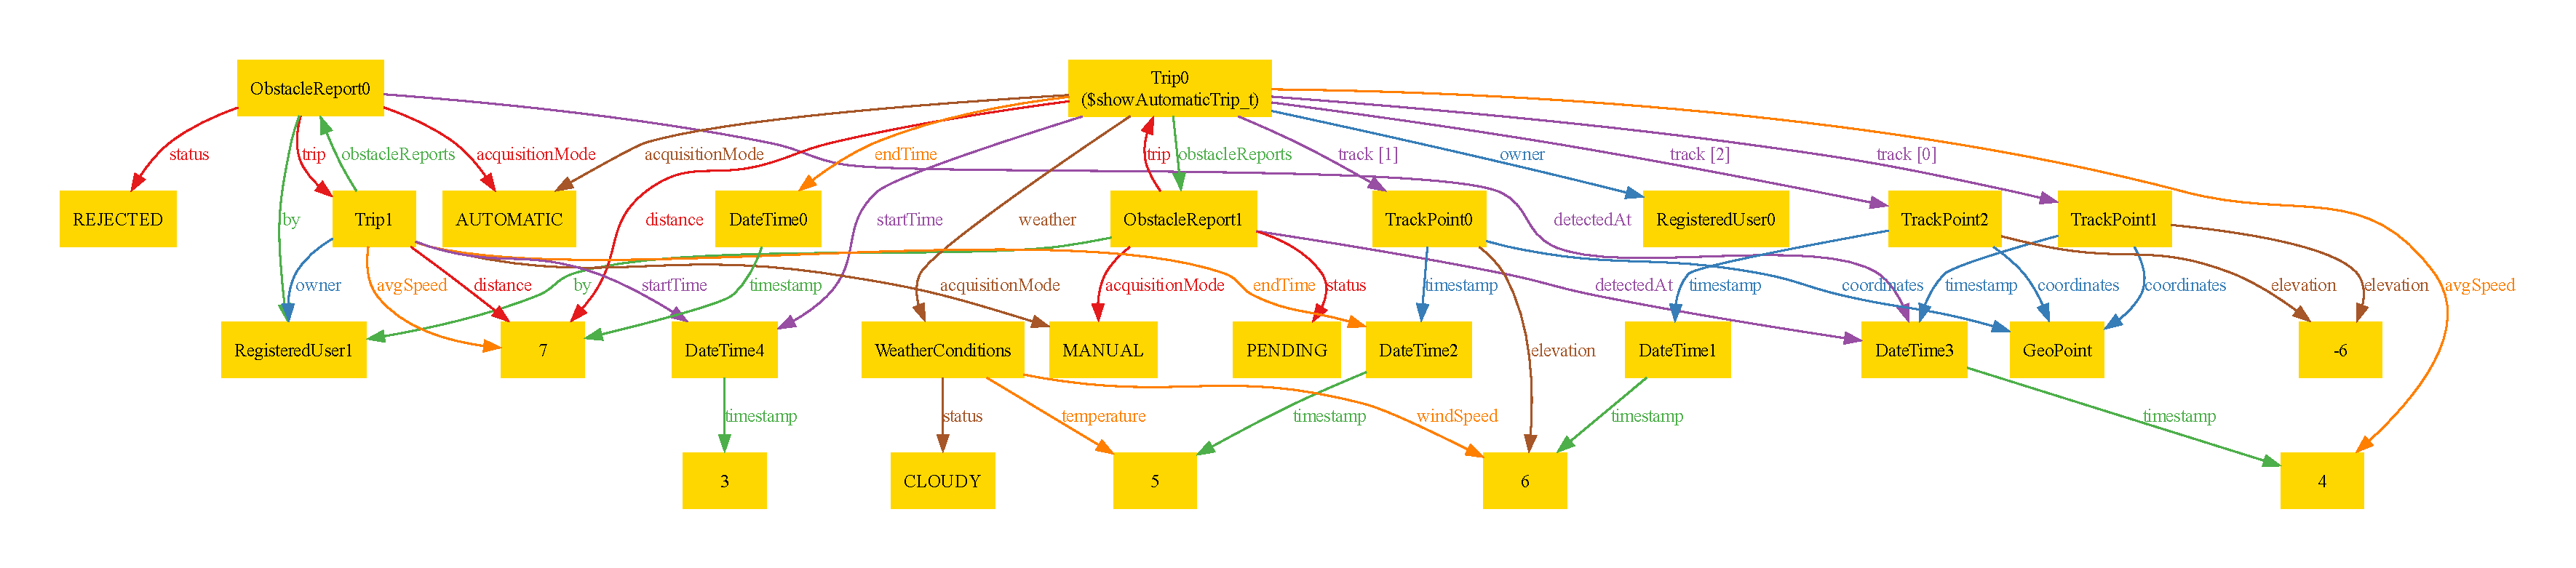
\includegraphics[width=\paperwidth]{Images/Alloy_images/Alloy-1.pdf}
}

    \caption{Generated image for the \texttt{showAutomaticTrip} predicate}
    \label{fig:alloy-automatic-trip}
\end{figure}

\par
\textbf{Scenario 2: Obstacle Reporting Workflow.}
Figure \ref{fig:alloy-obstacle-workflow} displays an instance generated by the \texttt{showObstacleWorkflow} predicate. This scenario validates the system's ability to handle the three distinct states of obstacle reporting and their differing structural implications.

The diagram highlights three specific reports corresponding to the assertion logic:
\begin{itemize}
    \item \textbf{Confirmed State (Validated Hazard):} \texttt{ObstacleReport2} is marked with the status \texttt{CONFIRMED}. Consistent with the \texttt{confirmedReportsLinkToObstacle} fact, this report is the only one in the set linked to a concrete \texttt{Obstacle} atom. This signifies that the system has verified the existence of the hazard on the associated \texttt{Street}.
    \item \textbf{Pending State (Awaiting Verification):} \texttt{ObstacleReport4} is shown with the status \texttt{PENDING}. It represents a newly submitted report that is currently stored in the system but has not yet been linked to a confirmed \texttt{Obstacle} entity.
    \item \textbf{Rejected State (False Positive):} \texttt{ObstacleReport3}, submitted by \texttt{RegisteredUser1}, holds the status \texttt{REJECTED}. As required by the \texttt{notConfirmedNoObstacleLink} fact, this report is isolated from any \texttt{Obstacle} atom, ensuring that invalid reports do not pollute the map data.
\end{itemize}

The scenario also demonstrates the integration of these reports within the broader environment, showing active \texttt{BikePath}s (e.g., \texttt{BikePath0}) and concurrent environmental factors.

\begin{figure}[H]
    \centering
    \makebox[\textwidth][c]{%
  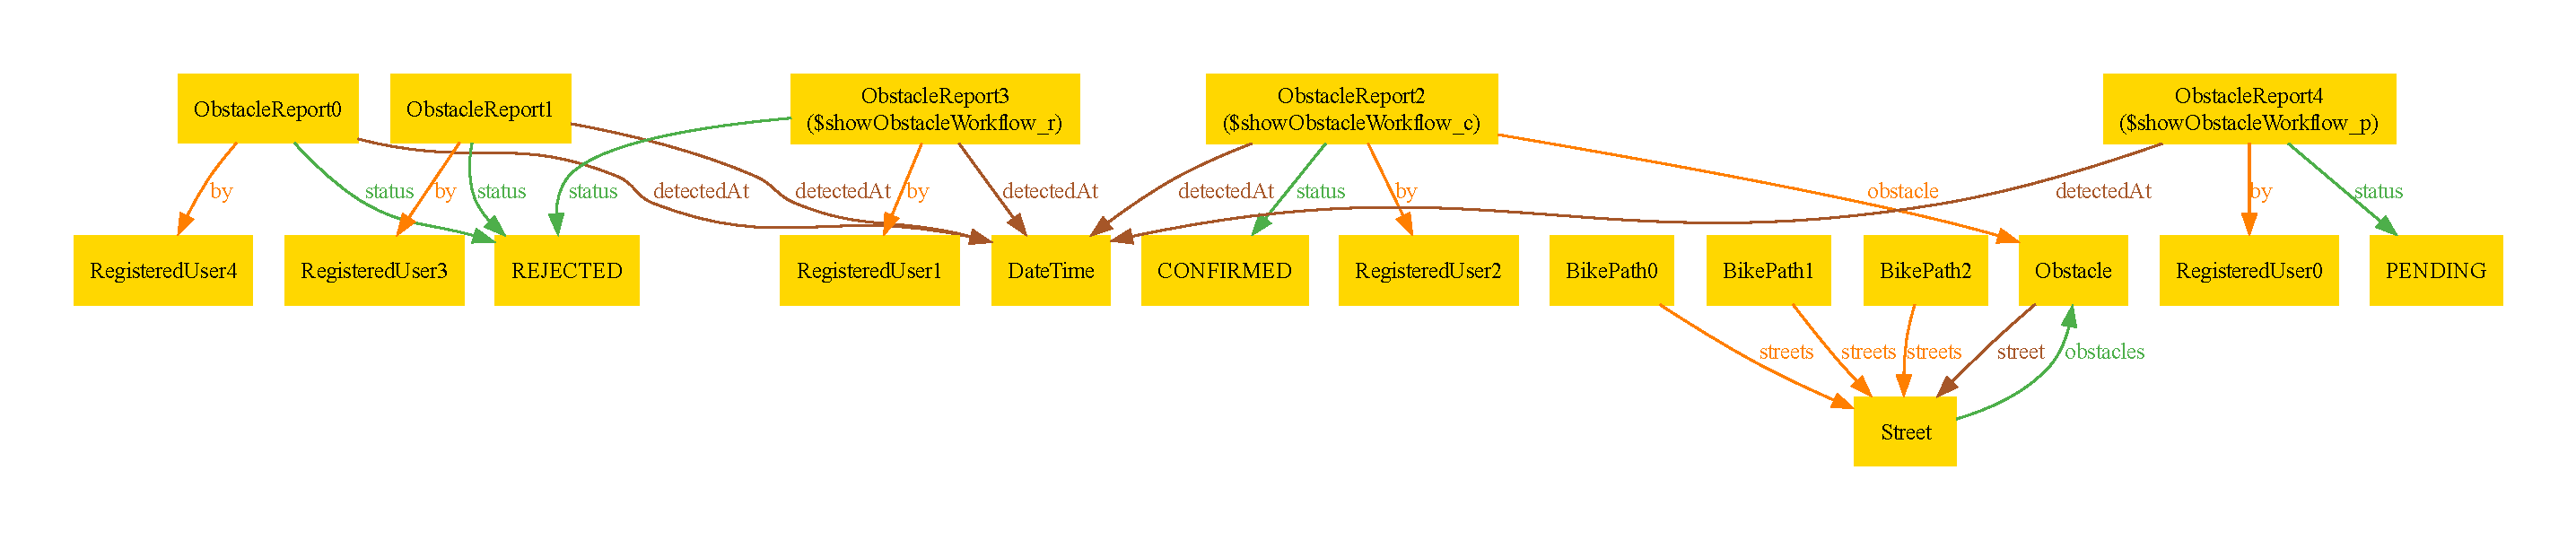
\includegraphics[width=\paperwidth]{Images/Alloy_images/Alloy-2.pdf}
}

    \caption{Obstacle workflow instance showing the coexistence of Pending, Confirmed, and Rejected reports, where only the confirmed report is linked to a physical Obstacle.}
    \label{fig:alloy-obstacle-workflow}
\end{figure}

\par
\textbf{Scenario 3: Path Status Merging.}
Figure \ref{fig:alloy-path-merging} illustrates the aggregation logic generated using the \texttt{showPathMerging} predicate, while enforcing the global bikePathStatusMerging constraint. The central entity is \texttt{BikePath2}, which is associated with multiple conflicting reports submitted by users.

The instance demonstrates the "Majority Rule" logic defined in the system's requirements:
\begin{itemize}
    \item \textbf{Conflicting Inputs:} The path is linked to three distinct reports via the \texttt{pathReports} relation:
    \begin{itemize}
        \item \texttt{PathStatusReport0} and \texttt{PathStatusReport2} both indicate the status is \texttt{SUFFICIENT}.
        \item \texttt{PathStatusReport1} indicate the status is \texttt{MEDIUM}.
    \end{itemize}
    \item \textbf{Majority Resolution:} Consistent with the \texttt{bikePathStatusMerging} fact, the system calculates the mode of the submitted reports. Since "Sufficient" has the majority count (2 vs 1), \texttt{BikePath2} is assigned the status \texttt{SUFFICIENT}.
    \item \textbf{Data Integrity:} All reports are correctly linked to a \texttt{RegisteredUser} and a \texttt{DateTime} timestamp, ensuring that the merging algorithm operates on valid, traceable data entries.
\end{itemize}

The scenario also confirms that this logic operates correctly within a larger context, as \texttt{BikePath2} coexists with other paths (\texttt{BikePath0}, \texttt{BikePath1}) and global \texttt{WeatherConditions} (shown as \texttt{SNOWY}), without structural conflicts.

\begin{figure}[H]
    \centering
\makebox[\textwidth][c]{%
  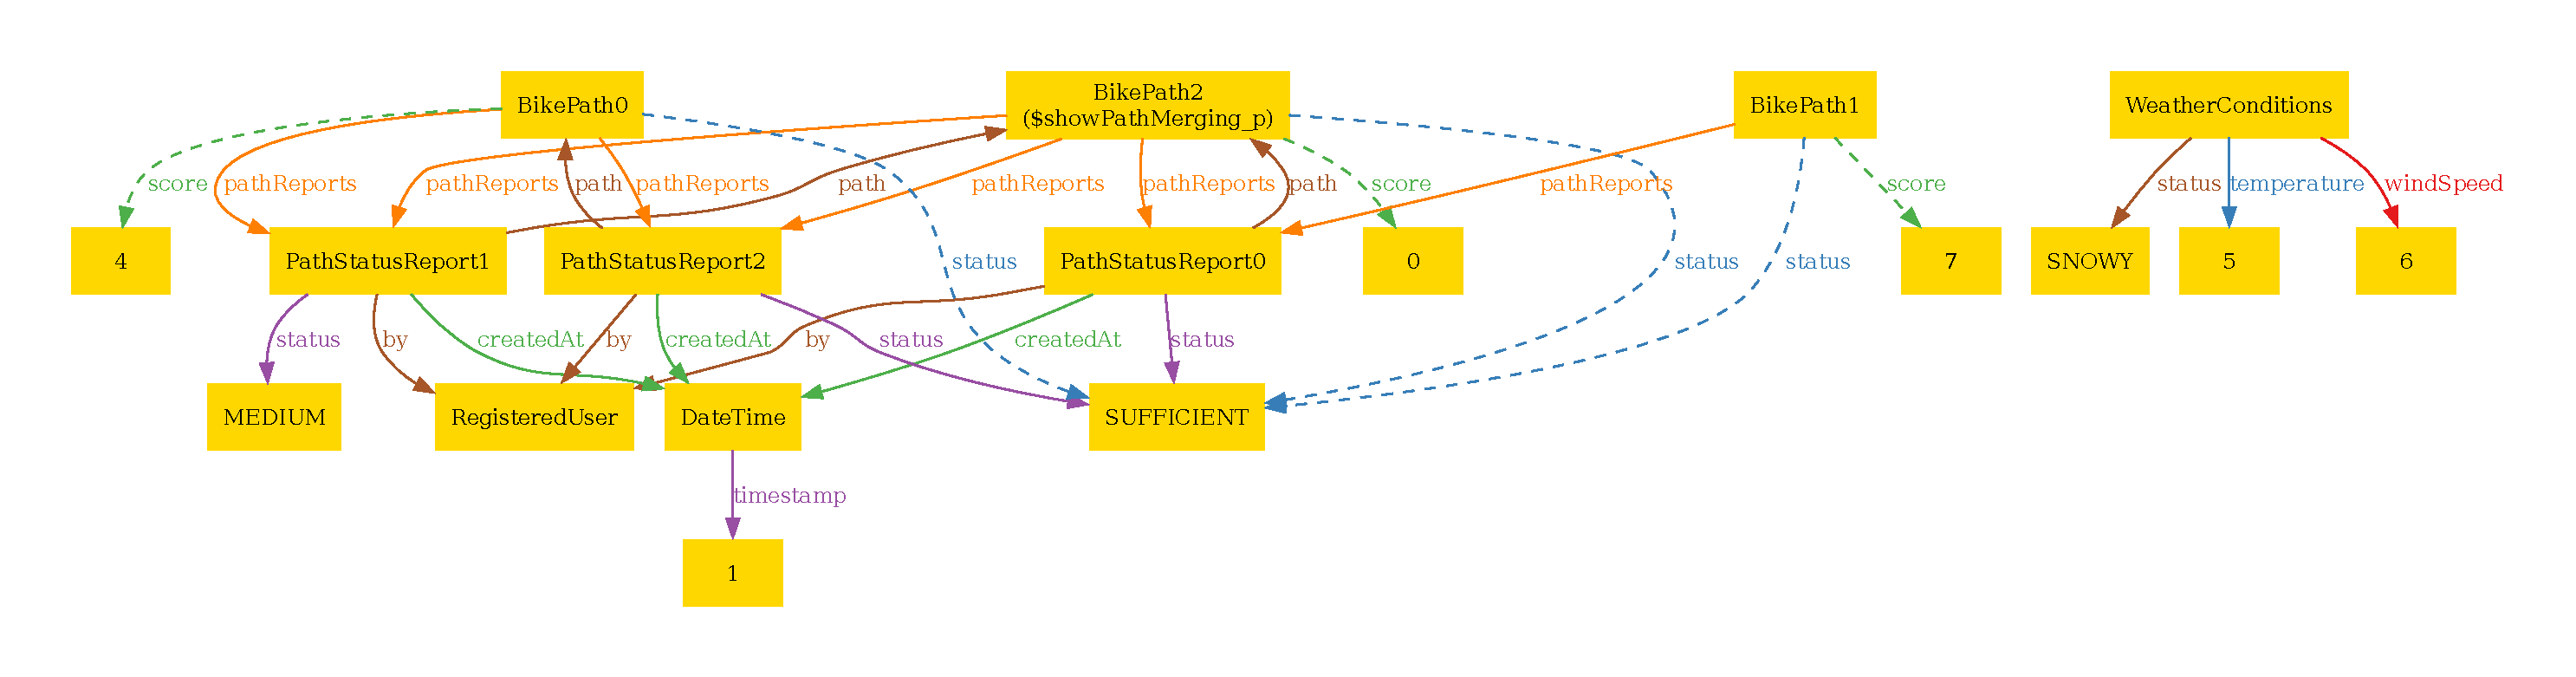
\includegraphics[width=\paperwidth]{Images/Alloy_images/Alloy-3.pdf}
}
    \caption{Path Merging instance showing \texttt{BikePath2} resolving a status of MEDIUM based on the majority of incoming user reports.}
    \label{fig:alloy-path-merging}
\end{figure}

\par
\textbf{Scenario 4: Comprehensive System State.}

Figure \ref{fig:alloy-complete-scenario} depicts a complete world generated by the \texttt{showCompleteScenario} predicate, capturing the simultaneous presence and interaction of trips, obstacle reporting, path status evaluation, and environmental conditions within a single consistent system state.

The instance highlights the following integrated aspects:

\begin{itemize}
    \item \textbf{Dual Acquisition Modes Across Multiple Entities:}  
    Both \texttt{MANUAL} and \texttt{AUTOMATIC} acquisition modes coexist and are applied consistently across different system components.
    \begin{itemize}
        \item \texttt{Trip1} is an \texttt{AUTOMATIC} trip, associated with weather information and enriched with an ordered sequence of GPS track points (\texttt{TrackPoint0}, \texttt{TrackPoint1}, \texttt{TrackPoint2}), each providing spatial, temporal, and elevation data.
        \item \texttt{Trip0} is a \texttt{MANUAL} trip. It records ownership, temporal bounds, distance, and average speed, but, consistently with the model constraints, it is not associated with any track points.
    \end{itemize}

    \item \textbf{Obstacle Reporting Lifecycle:}  
    The system includes multiple \texttt{ObstacleReport} instances with different acquisition modes and statuses.
    \begin{itemize}
        \item \texttt{ObstacleReport0}, acquired automatically during \texttt{Trip1}, is marked as \texttt{CONFIRMED} and is correctly linked to a physical \texttt{Obstacle} located on a \texttt{Street}.
        \item \texttt{ObstacleReport1} is a manually submitted report with status \texttt{REJECTED}.
        \item \texttt{ObstacleReport2} is also manually submitted and remains in the \texttt{PENDING} state.
    \end{itemize}
    All obstacle reports are associated with a registered user and explicit detection timestamps.

    \item \textbf{Path Status Reporting and Aggregation:}  
    A single \texttt{BikePath} is defined by an origin and a destination \texttt{GeoPoint} and is associated with the same \texttt{Street} hosting the obstacle.
    The bike path receives multiple \texttt{PathStatusReport} instances:
    \begin{itemize}
        \item \texttt{PathStatusReport0} is acquired automatically and reports a \texttt{MEDIUM} status.
        \item \texttt{PathStatusReport1} is acquired manually and reports a \texttt{SUFFICIENT} status.
    \end{itemize}
    These reports are created by a registered user and include creation timestamps. The bike path aggregates this information into a single path-level status of \texttt{MEDIUM}, along with a numerical score.

    \item \textbf{Environmental Context:}  
    The system state also includes environmental conditions through a \texttt{WeatherConditions} instance with status \texttt{SNOWY}, temperature, and wind speed. These conditions are explicitly linked to \texttt{Trip1}, demonstrating the integration of contextual data into trip-level information.
\end{itemize}

\begin{figure}[H]
    \centering
    \makebox[\textwidth][c]{%
  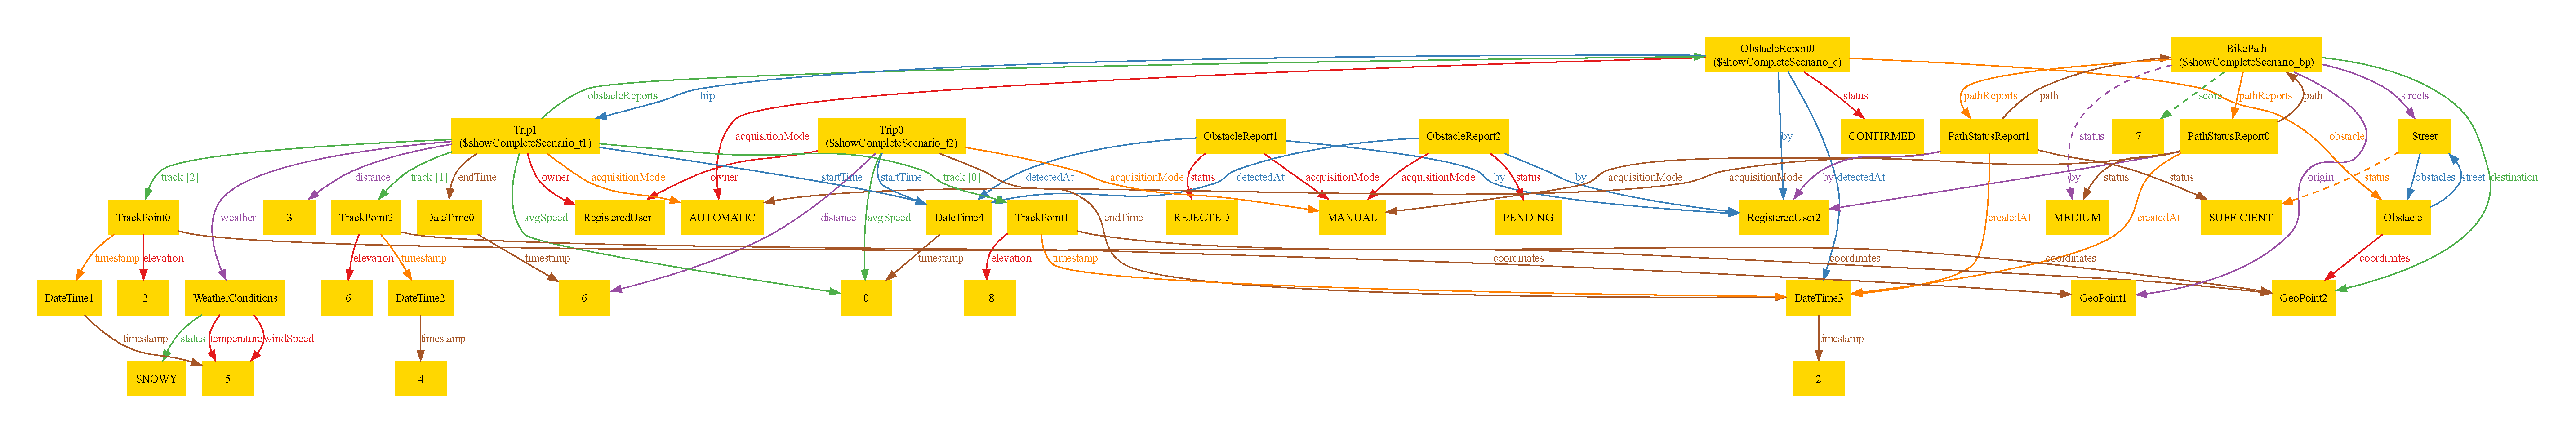
\includegraphics[width=\paperwidth]{Images/Alloy_images/Alloy-4.pdf}
}

    \caption{Complete scenario instance showing the coexistence of automatic and manual trips, obstacle reporting with different validation states, path status aggregation, and environmental conditions.}
    \label{fig:alloy-complete-scenario}
\end{figure}


\par
\textbf{Scenario 5: Path Status Majority Voting.}

Figure \ref{fig:alloy-majority-win} illustrates the instance generated by the \texttt{majorityShouldWin} predicate, which is designed to validate the resolution of conflicting path status reports through a majority-based aggregation strategy.

The diagram focuses on \texttt{BikePath1}, which is associated with three independent path status reports:

\begin{itemize}
    \item \textbf{Conflicting Status Reports:}
    \begin{itemize}
        \item \texttt{PathStatusReport1} and \texttt{PathStatusReport2} both assign the status \texttt{OPTIMAL} to the path.
        \item \texttt{PathStatusReport0} assigns a lower-quality status, namely \texttt{MEDIUM}.
    \end{itemize}

    \item \textbf{Majority-Based Aggregation Result:}  
    According to the majority voting logic enforced by the model, the system selects the most frequently reported status among those associated with the path. Since \texttt{OPTIMAL} appears twice out of three reports, \texttt{BikePath1} is assigned the aggregated status \texttt{OPTIMAL}, together with a corresponding numerical score.

    \item \textbf{Heterogeneous Data Sources:}  
    The three reports originate from different registered users (\texttt{RegisteredUser0} and \texttt{RegisteredUser1}) and employ heterogeneous acquisition modes:
    \begin{itemize}
        \item \texttt{PathStatusReport0} and \texttt{PathStatusReport1} are acquired in \texttt{AUTOMATIC} mode.
        \item \texttt{PathStatusReport2} is acquired in \texttt{MANUAL} mode.
    \end{itemize}
    This demonstrates that the aggregation mechanism operates independently of both the reporting user and the acquisition modality.

    \item \textbf{Contextual Information:}  
    For completeness, the scenario also includes environmental context through a \texttt{WeatherConditions} instance with status \texttt{SNOWY}, as well as a \texttt{Street} associated with the bike paths. These elements remain orthogonal to the voting process and do not influence the outcome of the majority decision.
\end{itemize}

\begin{figure}[H]
    \centering
  \makebox[\textwidth][c]{%
  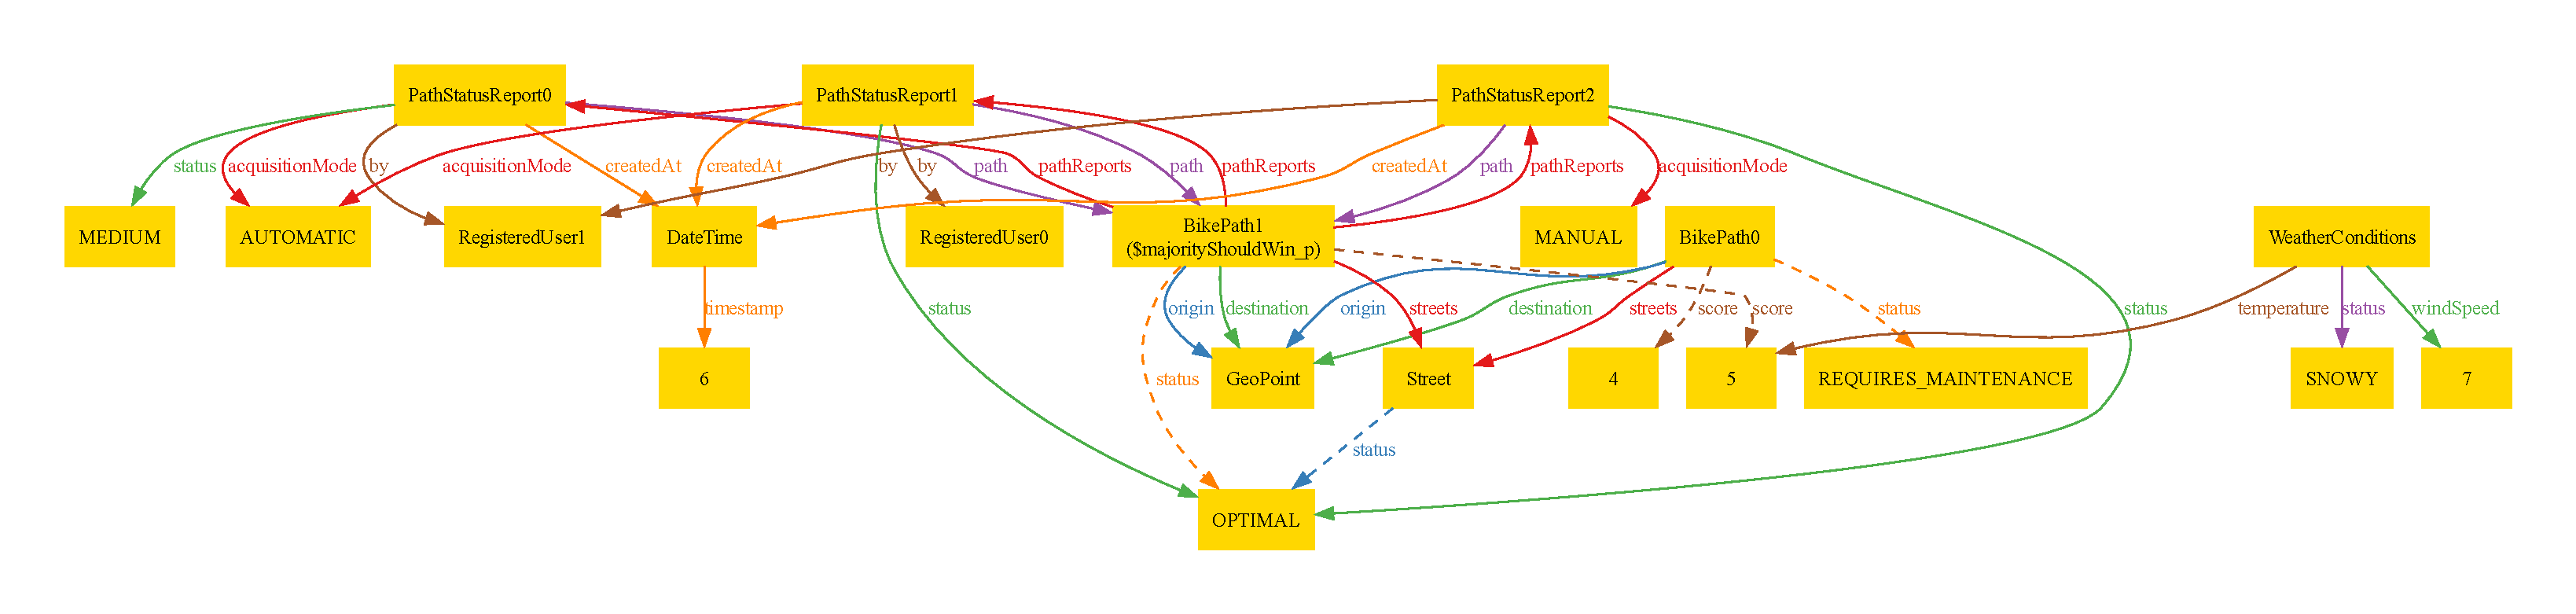
\includegraphics[width=\paperwidth]{Images/Alloy_images/Alloy-5.pdf}
}

    \caption{Majority voting scenario in which two \texttt{OPTIMAL} reports override a single \texttt{MEDIUM} report, resulting in an aggregated \texttt{OPTIMAL} status for the bike path.}
    \label{fig:alloy-majority-win}
\end{figure}
